\documentclass[main.tex]{subfiles}
\ProvidesPackage{preamble}

\usepackage[nottoc]{tocbibind}
\usepackage[english]{babel}
\usepackage[utf8]{inputenc}
\usepackage[table]{xcolor}
\usepackage[nohead, nomarginpar, margin=1in, foot=.25in]{geometry}
\usepackage{tabularx}
\usepackage{graphicx}
\usepackage{float}
\usepackage[english]{babel}
\usepackage{paralist}
\usepackage{datetime}
\usepackage{afterpage}

\begin{document}

\section{Background and Competitors}

The following sections provide a discussion of our defined target audience (identified with the help of User Types) and an in-depth analysis of competing backtesting tools.

\subsection{User Types}

During the process of identifying user types, we mainly relied on the methodology described in \cite{pathy}. In addition, the advice given by \cite{uiux_fundation} and \cite{user_types_interaction_design_fundation} proved invaluable. We began by gathering as much data as possible about the categories of people interested in backtesting and consequently in investing. The next step was to create several skeleton personas \cite{personas} and to validate their legitimacy through discussion with the team and cross-referencing with information gathered about various types of investors. Based on this, we decided that the creation of four personas would cover the vast majority of our target demographics.
These four personas created are described here with the full charts attached to this document in appendix \ref{user_types}.
\begin{itemize}
\item \textbf{Addriana: }Addriana is a 56-year old flower shop owner who is trying to invest in order to gain a comfortable retirement. She has previously used the services of a financial advisor but was left disappointed. As a result, she wants to have more control and more hands-on knowledge of the investments she is making.
\item \textbf{Allison: }Allison is a finance student in her 20s who wants to use the knowledge she acquired from university in a way that would allow her to both make a profit and gain insights to help in her career.
\item\textbf{Sam: }Sam is an accomplished middle-aged man who wishes to know more about investing and the benefits and disadvantages that come with it. 
\item\textbf{Timmy: }Timmy is a high-school student who is interested in short term investments. He would describe himself as being part of the new wave of cryptocurrency enthusiasts.
\end{itemize}

With the personas created, we conceived of a number of scenarios where backtesting could be of value. We then put each persona in turn through them. This process helped us to extract the empathy maps \cite{empathy_maps} of our personas. We then validated our empathy maps with our team and with outsiders to provide a third party perspective. The validation with people from outside the team proved to be crucial in adjusting for internal biases.
Based on the user personas and their empathy maps, we then began looking at what types of metrics we could best use to describe them. We identified the critical ones to be the knowledge on the topic of finance and the amount of funds available for investing. Another metric that was found to be important was that of the various types of investing timeframes (differentiating between users aiming at short or long term investments). Based on these metrics, we identified the following four user types:

\begin{enumerate}
    \item \textbf{Financial Proficiency and Large amounts of Capital:  }This person already knows the benefits of backtesting and is only looking for a tool that can speed up the process of constructing an investment portfolio. The resources they have meant that they would likely be able to afford our product with ease. This type of user would likely engage in both long and short term investments.
    \item \textbf{High Financial Knowledge and Little Capital:  } This is most likely someone young who has a keen interest in finance or is studying it at a university. Price could be a deterrent for them if their main aim is to conduct short term investing. If they would be doing long term investing, however, the price would likely not pose a problem as they would consider it a necessary part of their initial investment.
    \item \textbf{Little Financial Knowledge and Large amounts of Capital:  }This is a person who wants to switch from having a savings account or employing a financial advisor. They are aware of the learning curve and need additional information before they are willing to commit to any major decisions. They will be happy to pay for our product in order to gain access to our data, analysis and general advice.
    \item \textbf{Little Financial Knowledge and Little Capital:  }This last category is made up of individuals who lack confidence in their ability to invest successfully. As a result, they do not want to risk large sums of money until they are sure that they can make the right decisions. There is a good chance that they will purchase our product to form a clearer idea of what investing as an activity consists of. After gaining confidence and experience they will likely increase the funds they are comfortable investing.
\end{enumerate}


\subsection{Competitor Analysis}

As a result of our initial competitor analysis, we can group competing software into two categories. For a comprehensive list of available backtesters, see \cite{listofbacktesters}. The first category is that of full-suited trading software, such as Fidelity Active Trader Pro \cite{Fidelity}, MetaTrader4 \cite{MetaTrader} and NinjaTrader \cite{NinjaTrader}, which offer backtesting as an additional feature. Services in this category focus on features such as the buying and selling of financial assets, prediction of future prices and storage and management of a user's capital. Although it may be beneficial to consider some features related to real time trading, these would only be part of a future development process and are not within the scope of our prototype.

The second category consists of software that does not offer trading as a service and instead focuses solely on backtesting. Thus, for now, we shall only consider the feature set provided by the second category, as it is directly comparable to the service we are aiming to provide. In the following paragraphs, we will consider some of the design decisions made by competing software, together with a brief analysis and conclusion on each feature.

\subsubsection{Portfolio Visualizer}
Our main competitor of the second category is an online backtesting tool named Portfolio Visualizer \cite{portfoliovis}. During the inception phase of development, we relied heavily on this website for requirement analysis and elicitation. Let us now briefly dissect what it has to offer. 

Upon opening the website we are greeted with a brief description of the domain, together with the following input form:

\begin{figure}[H]
   \centering
   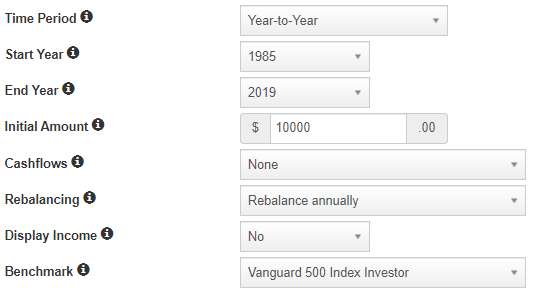
\includegraphics[scale=0.8]{02Background/02Pictures/portfolio_visualizer_input_1.png}
   \caption{Portfolio Visualizer - Input (source: https://www.portfoliovisualizer.com/)}
\end{figure}

As we can already see, the key elements of portfolio analysis are provided. Considering the functionality of our prototype as a baseline (i.e. testing an allocation of assets with a fixed initial investment over a fixed time period), we see that in addition, users are able to perform the following set of actions:

\begin{itemize}
  \item Set the endpoints of the investment period, up to months.
  \item Set the initial investment. 
  \item Specify a regular cash flow and its frequency.
  \item Select a rebalancing strategy.
  \item Select a benchmark strategy for comparison.
  \item Compare multiple strategies at the same time.
  \item Adjust for inflation.
  \item Select from a set of lazy portfolios (benchmarks).
  \item Calculate additional metrics.
  \item Export the results to PDF, Excel, or save a link. 
\end{itemize}

At first, it may seem as if Portfolio Visualizer meets all the requirements needed for a backtesting tool. Indeed, our main criticism is with respect to the UI, responsiveness and user experience, findings based on our initial user testing. 

The UI design is simplistic and has a non-commercial, bare-bones look. Although this was appreciated while testing the system, it certainly does not improve the user experience. The input, mostly using dropdown menus, is straightforward to use, except for the selection of assets, which we will discuss briefly at the end of this section.

% This did not age well
% Moreover, users will want to fine-tune their investment strategies by changing their allocations frequently. The only means to do this when using Portfolio Visualizer is to scroll to the top, change the input and rerun the entire simulation. Our goal is to design a more responsive and dynamic system, to ease this procedure. 
% It certanly did not

The website also supports user accounts. However, little to no data is associated with a user's profile, which further decreases the overall user experience. Finally, as a last remark, which holds for most of the backtesting tools we have tried, the website displays a heavy US bias and hence the selection of asset classes is limited.
% Furthermore, we have no means of changing the currency, which would also be an important feature for a product accessible through the web (and therefore available to users from all over the globe).

\subsubsection{Other Competing Software}

The rest of the alternatives are of a significantly lower quality. In the remaining parts of this section, we will briefly consider a few design decisions made by these websites.

\subsubsection*{Tree-like Asset Selection}

One challenging aspect of designing such a system is summarised by the following question: 

\begin{quote}
    What is the most intuitive way for selecting a portfolio item? 
\end{quote}

Where a portfolio item could be: an equity, ETF index, a commodity, bond, or the like. Within each of these classes there are many more options to choose from. Many backtesters opted for a search bar, which is a sensible approach. Nevertheless, many portfolio items are named similarly, and for a new user, it is a high barrier to entry as they might not know what is available. 

Another option is what ETFReplay \cite{etfreplay} has implemented, which is a tree-like selection form, shown below. 

\begin{figure}[H]
   \centering
   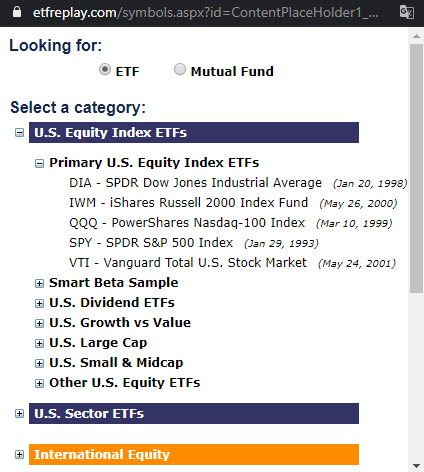
\includegraphics[scale=0.7]{02Background/02Pictures/etfreplay.png}
   \caption{ETFReplay - Tree-like Structure (source: https://www.etfreplay.com/)}
\end{figure}

However, pursuing this form of gathering input from the user involves multiple repetitive actions of expanding the tree structure, which becomes tedious once one is more familiar with the tool. Thus, we have chosen to pursue the search bar approach.

% We believe this was the most intuitive to use and will thus pursue a similar approach. The only potential issue associated with this is that it opens in a new window, which we would prefer to avoid.

\subsubsection*{Tiles}

It may be worth briefly discussing one example of a backtester with a good design. We found the simplistic and tiled design of Backtest Curvo \cite{backtestcurvo} a good choice, as it gives the website an overall modern and fresh look, whereas most backtesters looked old and out of date. Our goal is to achieve a layout similar to this. For a further analysis on design decisions, please see \ref{Design}.

\subsubsection*{Simple Scripting Language}

In our whitepaper, we briefly discussed implementing a simple scripting language which would allow users to simulate dynamic trading strategies \cite{WP}. As mentioned in our white paper, this would not be in the scope of the course, but for inspiration, we can have a look at the approach of Stockbacktest \cite{stockbacktest}.

\begin{figure}[H]
   \centering
   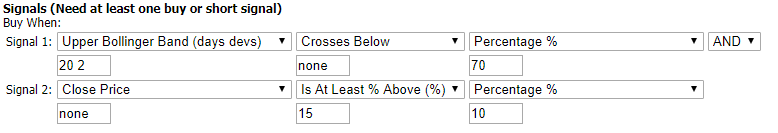
\includegraphics[scale=0.7]{02Background/02Pictures/stockbacktest.png}
   \caption{Stockbacktest - Simple Logic (source: http://stockbacktest.com/)}
\end{figure}

Although not intuitive at all, it demonstrates that this feature is possible to implement. We believe that after nailing down precisely how the user would create the rules, this would be a straightforward task, as the calculations involved are not more complicated than in the static case. As mentioned previously, this is something we would like to implement in the future.

\subsubsection{Summary}
\label{reliability}

After testing competitor software during the inception phase of development, we were left with three key observations. These were the following:

\begin{itemize}
    \item Transparency: Many of the testers' web pages did not give the impression of being operated by a reputable business. In the worst case, they gave the impression of being nontransparent or untrustworthy (misspelt words, advertisements with questionable subject matter), which is something we should avoid.
    \item Learning Curve: After getting to know our target audience, we concluded that most seem willing to learn how to use a complex system, if they believe it is worth it.
    \item Design of the UI: It was easy to tell which backtesters are still getting updated by looking at their design. We should aim at providing a fresh design. In addition, some backtesters offered so many features that every corner of their UI was packed with information. This is something we should also avoid doing.
    %In west Philladelphia, born and raised ~
    
\end{itemize}

The analysis was conducted informally with the help of colleagues studying or otherwise involved in finance. This allowed us to develop a more neutral and accurate impression, despite the subjective nature of the observations. Having analysed the competing software, we are now better suited to determine the requirements of our system. 

\end{document}
